\chapter{Testautomatisierung mit Selenium}
\label{sec:testautomatisierung_mit_selenium}
Die Benutzeroberfläche ist als Schnittstelle für die Testautomatisierung weit verbreitet. Hierfür gibt es mehrere Gründe. Die Benutzeroberfläche ist sowohl für Tester als auch für den Entwickler leicht greifbar und sehr anschaulich. Testfälle die über die Benutzeroberfläche arbeiten kommen dem realen Verwendung der Anwendung sehr nahe und die Dokumentation ist auf dieser Ebene meist am vollständigsten. Wird die Benutzeroberfläche für die Automatisierung verwendet kommt das Vorgehen dem von klassischen Systemtests sehr nahe, da diese zumeist über die selber Schnittstelle durchgeführte werden. \cite[vgl. Seite 48]{seidl_basiswissen_2012} Das fördert vor allem die Akzeptanz des Testautomatisierungsprojektes auf der Fachseite da schnell sichtbare Erfolge erzielt werden können. 
Ein weit verbreitetes Tool für die Automatisierung von Tests gegen die Benutzeroberfläche ist Selenium.

\section{Selenium}
\label{sec:selenium}
Selenium \cite{selenium_selenium_????} ist eines der am weitesten verbreiteten Open-Source-Automatisierungswerkzeuge für Webapplikationen. Ordnet man das Tool gegen die in Kapitel \ref{sec:möglichkeiten_zur_testautomatisierung_in_erstellung_und_durchführung} beschirebene Unterteilung der Testautomatisierung ein, befinden sich Selenium in den unteren beiden Quadranten.
Selenium ist also ein Tool das sowohl das manuelle Skripten von UI Tests wie auch das halbautomatische recorde-and-playback unterstützt. Selenium ist genaugenommen aber kein einzelnes Tool. Der Begriff steht eher für eine Reihe von Komponenten mit unterschiedlicher Funktionalität die der Testautomatisierung dienen. Dabei können folgende Teile unterschieden werden:

\begin{itemize}
	  \itemsep0pt
      \item \textbf{Selenium IDE} (Integrated Development Environment), eine Firefox-Extension, welche eine recorde-and-playback Funktionalität beinhaltet. Mit der Selenium IDE ist es möglich Browserinteraktionen aufzuzeichen und die so erstellten Skripte zu editieren.
      \item \textbf{Selenium Core} enthält die komplette Basisfunktionalität von Selenium, also das Testbefehl-API und den TestRunner. Mit Hilfe des Selenium Core können aufgenommene Skripte später wieder abgespielt werden.
      \item \textbf{Selenium WebDriver} ermöglicht es, Selenium aus Skripten und Programmiersprachen zu verwenden. Der WebDriver bietet dazu eine API die es ermöglicht mit unterschiedlichen Browsern zu kommunizieren.
      \item \textbf{Selenium Grid} für die Parallelisierung von Testdurchläufen.     
\end{itemize}

Was Selenium also bietet, ist eine Reihe von Komponenten die der Testautomatisierung in den Bereichen Testcodeerstellung \ref{subsec:testcodeerstellung} und Testdurchführung \ref{subsec:testdurchf\"uhrung} liegen

\section{Testdesign mit Selenium}
\label{sec:Testdesign}
Selenium bietet kein Werkzeug das den Tester in der Designphase des Testprozesse unterstützt.
Es ist mit Selenium also nicht möglich automatisiert Testfälle generieren zu lassen. Entscheidet man sich für Selenium als Testautomatisierungslösung werden die Testfälle in der Regel wie in Kapitel \ref{subsec:testanalyse_und_design} Testanalyse und Design beschrieben manuell erstellt. Selenium unterstützt zwar nicht den Desingprozess von Testfällen , versperrt jedoch auch nicht eine mögliche Automatisierung. Werden Testfälle, wie in Kapitel \ref{subsec:testanalyse_und_design} beschrieben, automatisch erstellt könne sie durchaus später mit Hilfe von Selenium automatisiert werden. Beispielsweise wäre ein Datengetriebener Automatisierungsansatz mit zuvor generierten Testeingaben durchaus denkbar. Das Zusammenspiel von beiden Phasen, also das automatische designen von Testfällen für die auch gleich automatisiert die Testskripte generiert werden, wie es beispielsweise modellbasierte Ansätze ermöglichen, ist jedoch ohne weiteres nicht möglich.

\section{Testcodeerstellung mit Selenium}
\label{sec:Testdesign}

Im Bereich von GUI-Applikationen stellen Webanwendungen einen Spezialfall dar. Anders als in den meisten Denktopanwendungen ist die Kernfunktionalität der Anwendung Serverseitig realisiert. Als Kommunikationsschnittstelle zwischen Clients und Server dient HTML. Die eigentliche Benutzeroberfläche wird erst auf Clientseite durch den Browser aus dem gelieferten HTML-Dokument erzeugt. Das bietet für Testtools eine gute Basis, um auf die Elemente der Benutzeroberfläche zuzugreifen. \cite[vgl. Seite 59]{seidl_basiswissen_2012} UI-Testtools für Desktopanwendungen haben oft mit großen Herausforderungen zu kämpfen um die einzelenen Grafikelemente einer Anwendung zu identifizieren. Selenium kann hier einfach auf Browserfunktionalitäten bzw. auf die Struktur der HTML-Seite (Document Object Model), zurückgreifen. Über das Document Object Model können Tester die einzelnen Elemente einer Seite identifizieren und Interaktionen mit ihnen durchführen. Auf diese Weise kann der Workflow eines Testfalls in der Anwendung nachgebildet werden.

Selenium bietet dafür zwei unterschiedliche Möglichkeiten. Der Testcode zum abbilden des Workflows kann halb automatisiert über eine recorde-and-playback Funktionalität oder manuell erstellt werden.

\subsection{Recorde-and-playback}
\label{sec:recorde_and_playback}
Das automatisierte Aufnahme von Testfällen ist eine der wichtigsten Funktionen der
Selenium IDE. Befindet sich die IDE im Aufnahmemodus werden alle Interaktionen des Benutzers mit dem Browser gespeichert. Das so erstellte Testskript wird in einer Selenium eigenen Sprache gespeichert. Diese Sprache wird Selenese genannt. Die einzelnen Selenese-Kommandos werden in einer HTML-Tabellenstruktur abgelegt. Diese Tabellen mit Selenese-Kommandos können später wieder verwendet werden um den gespeicherten Workflow erneut zu durchlaufen.
Selenium leidet jedoch unter den selben Problemen unter denen die meisten recorde-and-playback-Tool leiden. Aufgenommene Testfälle sind in der Regel instabil.
Um die einzelnen Elemente der Website zu identifizieren benutzt Selenium das Document Object Model der Website. Schon kleine Änderungen an der Oberfläche oder leicht veränderte Testdaten können die Struktur der Seite so stark verändern, dass die Testfälle die gespeicherten Elemente nicht mehr identifizieren können. Über die recorde-and-playback Funktionalität erstellte Testfälle erfordern daher eine vorgelagerte Planungs- und nachgelagerte Nachtbearbeitungsphase um die Testskripte auch für nachfolgende Durchläufe robust zu machen. Diese vorgehen widerspricht aber dem eigentlichen Grundgedanken von recorde-and-playback, der darauf abzielt, die Testskripterstellung möglichst einfach und schnell zu gestalten.
Benutzt man für die Testskrtipterstellung die recorde-and-playback Funktionalität der Selenium IDE ist man nicht an die Sprace Selenese gebunden. Die IDE bietet die Funktionalität die in Selenese erstellten Testskripte in eine Reihe von verschiedenen Programmiersprachen zu exportieren.
Die so erstellten Testskripte sind in ihrem Aufbau identisch zu den Testskripten die in Selenes generiert wurden und basiert immer auf einem xUnit-Framework der ausgewählten Sprache.
Sie leiden daher auch unter der selben Instabilität unter der bereits die Selenes Testfälle leiden. Darüber hinaus ist generierte Testcode wenig gekapselt und schwer wiederverwendbar. Das macht die generierten Skripte sehr Wartungsaufwändig und schlecht lesbar.
Diese Funktionalität sollte daher eher als Prototyping von Skripten verstanden werden.


\subsection{Manuell}
\label{sec:manuell}
Eine andere Möglichkeit ist das manuelle programmieren der Testskripte. Der manuell erstellte Testcode bedient sich den selben Tools die auch die Generierten und Exportierten Testfälle aus der recorde-and-playback Variante verwenden. Das macht die Testfallerstellung zu beginn im Vergleich zur halbautomatischen Variante aufwendig. Dieser Mehraufwand kann allerdings durch deutlich bessere Wartbarkeit und Wiederverwendbarkeit schnell wieder eingespart werden. Im Gegensatz du den generierten Testfällen kann bei einem manuellen Ansatz von Anfang an auf eine wartbare und wiederverwendbare Struktur in den Testfällen geachtet werden. Als best practice hat sich hierfür das Page Object Design Pattern \cite{selenium_test_????} durchgesetzt. Jede Maske der Anwendung wird als eigene Klasse umgesetzt. Diese Klassen beinhalten als einziger Ort in den Testskripten die Informationen über Funktionalität und Aufbau der Maske. So können redundanter code und redundante Informationshaltung vermieden werden. Die Wartbarkeit und Robustheit der Testskripte steigt.


\section{Testdurchführung mit Selenium}
\label{sec:testdurchführung_mit_selenium}

Testfälle die in mit Hilfe der recorde-and-playback Funktionalität aufgenommen wurden, können direkt über die Selenium IDE oder auch in Selenium Core, einem HTML-basierten Durchführungswerkzeug automatisiert ausgeführt werden. 
Manuell erstellte bzw. exportierte Testfälle bedienen sich zur Ausführung dem entsprechenden xUnit Framework der benutzten Programmiersprache. Im Fall von Java wäre das beispielsweise JUnit oder TestNG. Selenium setzt für die Ausführung also auf gut verbreitete Frameworks die im Bereich der Unit bzw. Integrationstests gegen die API-Schnittstelle bereist also Standartframeworks verwendet werden. Diese Frameworks sind den meisten Entwicklern bereits bekannt und gut in den Entwicklungsprozess integriert. In Java wird beispielsweise JUnit in allen gängigen IDEs durch Plugins unterstützt. Noch viel wichtiger ist jedoch, die bereits vorhandene Integration in den Buildprozess.
Hält man sich an Standarttools wie Maven oder Gradle zum bauen seine Projekte, können Testfälle die auf den gängigen xUnit-Frameworks basieren direkt in den Buildprozesse eingebunden werden.
Die automatisierte Ausführung der UI-Tests mit Selenium ist daher besonders einfach, da mit Standartmitteln möglich.

\section{Testabdeckung mit Selenium}
\label{sec:testdurchführung_mit_selenium}

Nach Abschluss der Tests stellt sich häufig die Frage: Wie gut sind meine Tests? Habe ich genug Testfälle oder benötige ich noch mehr? Um diese Fragen zu beantworten wird als Metrik häufig die Codeabdeckung durch die vorhandenen Testfälle herangezogen. Bei diesem Vorgehen wird gemessen wie viel Prozent der Codezeilen der zu testenden Anwendung bei der Ausführung der vorhandenen Testfällen durchlaufen wird.
In herkömmlichen Testfällen welche die API der Anwendung als Schnittstelle benutzen ist das recht einfach Möglich. Möchte man die Codeabdeckung seine Unittests messen, können in Java beispielsweise Tools wie EclEmma oder JaCoCo verwendet werden. Selenium verwendet als Schnittstelle allerdings nicht die API der Anwendung, sondern das UI. Das messen der Codeabdeckung ist in diesem Fall deutlich schwieriger. In der Regel wird gegen eine fertig gebaute Anwendung getestet. Dabei muss darauf geachtet werden, dass der durchlaufene Code in der Anwendung und nicht im Testprojekt gemessen wird.
Das erweist sich meist als deutlich schwierigere Aufgabe also das Messen beim verwenden der API. Das vorgehen ist stark von der Programmiersprache, in der die zu testende Anwendung entwickelt wurde und von den verwendeten Testtools abhängig. Im Java ist hierfür beispielsweise eine Bytcode Manipulation der zu testenden Anwendung notwendig, bei der jeder Klasse in der die Codeabdeckung gemessen werden soll die entsprechenden Anweisungen injiziert werden.


\chapter{Ausblick}
\label{sec:ausblick}

Das Thema Testautomatisierung wird auch in den kommenden Jahren ein wichtiges Thema im Bereich der Softwareentwicklung bleiben. Vor allem Continous Integration und Continous Delivery werden hier weiter eine Treibende Kraft sein. Diese zwei Bereiche sind als Entwicklungskonzepte derzeit sehr stark im Trend, was auch der Verlauf der Suchanfragen in den letzten Jahren zeigt.
\begin{figure}[htb]
  \centering  
  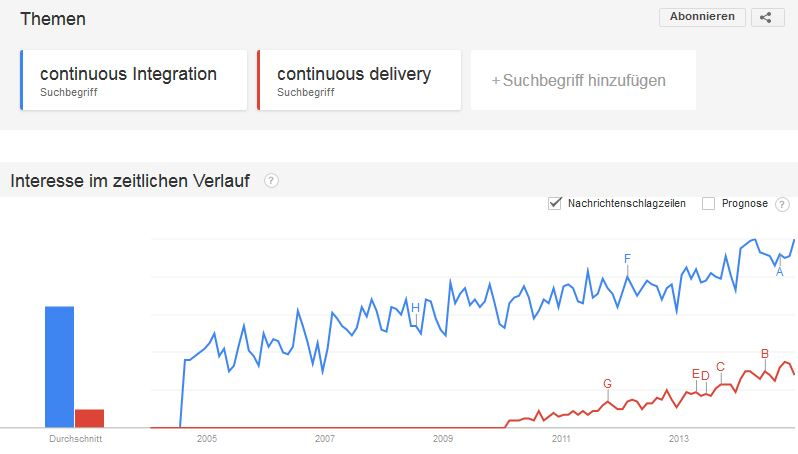
\includegraphics[scale=0.75]{img/cdTrend.JPG}\\
  \footnotesize\sffamily\textbf{Quelle:} \cite{google_google_2014}
  \caption{Trend der Suchanfragen nach dem Begriffen ‘continous integration‘ und ‘continous delivery‘ seit 2006}
  \label{fig:cdTrend}
\end{figure}
Die Testautomatisierung ist ein integraler Bestandteil dieser Entwicklungskonzepte und wird daher von diesem Trend mitgetragen werden. Unittests bzw. Integrationstests mit den gängigen XUnit-Frameworks haben sich bereits in vielen Projekten durchgesetzt. Für eine sinvolle Continous Integration bzw. Continous Delivery müssen jedoch alle Bereiche, von Unit- bis Systemtest durch eine Automatisierung abgedeckt werden. Es ist daher zu erwarten, dass auch die Automatisierung in diesen Bereichen für viele Projekte an Interesse gewinnen wird.


Im Bereich der Automatisierungstools wird Selenium auch in der nächsten Zeit eine weit verbreitete Lösung darstellen. Der Verlauf der Suchanfragen in den Letzten Jahren zeigt, dass Selenium im Vergleich zu anderen gängigen Lösungen immer noch sehr beliebt ist.

\begin{figure}[htb]
  \centering  
  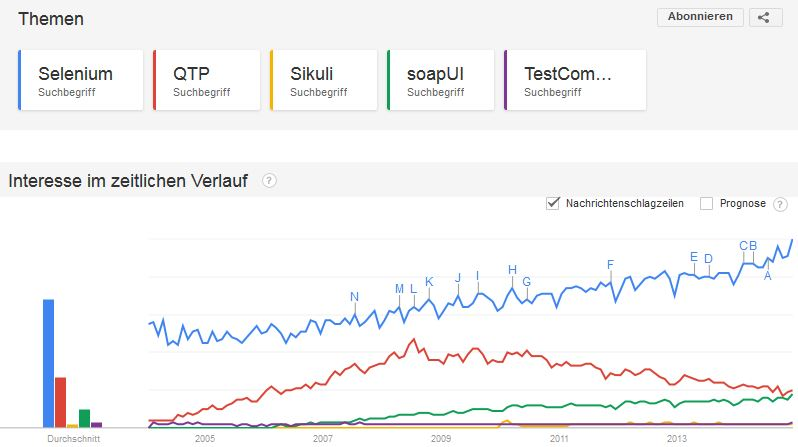
\includegraphics[scale=0.75]{img/autoToolsTrend.JPG}\\
  \footnotesize\sffamily\textbf{Quelle:} \cite{google_google_2014}
  \caption{Trend der Suchanfragen nach gängigen Automatisierungstools}
  \label{fig:cdTrend}
\end{figure}